\lesson{Atomic Theories}
\subsection{Dalton's Atomic Theory}
Matter is composed of indestructible, indivisible atoms, which are identical for one element,
but different from other elements. This model is commonly referred to as the \textbf{billiard ball model.}

\begin{tabularx-custom}{|X X|}{Creating the Dalton Atomic Theory (1805)}
    Key Experimental Work & Theoretical Explanation \\ \hline
    Law of definition composition: elements combine in a characteristic mass ratio
    & Each atom has a particular combining capacity \\ \hline
    Law of multicple proprtions: there may be more than one mass ratio & Some atoms have more
    than one combining capacity \\ \hline
    Law of conservation of mass: total mass remains & Atoms are neither created nor destroyed
    constant in a chemical reaction \\ \hline
\end{tabularx-custom}

\subsection{Thomson Atomic Model}
Thomson's quantitiative work with the cathode ray resulted in the discovery of the electron. 
Thomson was able to deflect the cathode ray towards a positively charged plate to deduce that the 
particles in the beam were negatively charged. Thomson's model is commonly referred as the 
\textbf{plum pudding model}. See Figure \ref{fig:thomson-cathode-ray}.

\begin{figure}[ht!]
    \centering
    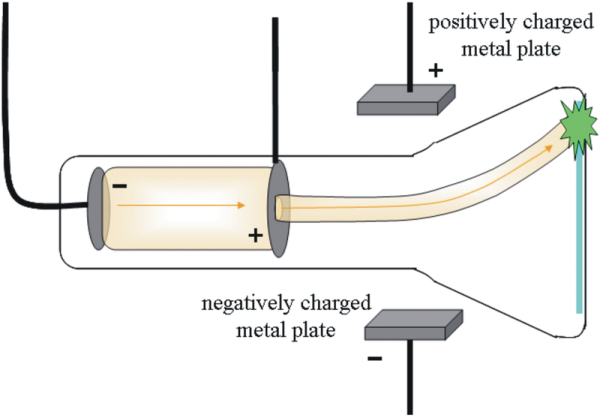
\includegraphics[width=0.6 \textwidth]{../figures/thomson-cathode-ray.png}
    \caption{The charged particles were directed in the direction of the positively charged
        plate, thus he concluded that these particles, which were smaller than the smalles atom,
        where negatively charged. A \textbf{cathode ray} is a stream of electrons.}
    \label{fig:thomson-cathode-ray}
\end{figure}

\begin{tabularx-custom}{|X X|}{Creating the Thomson Atomic Theory (1897)}
    Key experimental work & Theoretical explanation \\ \hline
    Arrhenius: the electrical nature of chemical solutions & Atoms may gain or lose electrons
    to form ions in solution \\ \hline
    Faraday: quantitative work with electricity and solutions & Particular atoms and ions gain
    or lose a specific number of electrons \\ \hline
    Crookes: qualitative studies of cathode rays & Electricity is composed of negatively charged
    particles \\ \hline
    Thomson: quantiative studies of cathode rays & Electrons are a component of all matter \\ \hline
    Milikan: charged oil drop experiment & Electrons have a specific fixed electric charge \\ \hline
\end{tabularx-custom}

\subsection{Rutherford Atomic Theory}
Rutherford used radium as a source of alpha radiation and directed it at a thin film of gold. \textbf{Note:}
it is kind of fortunate that Rutherford used gold because the nucleus is so large which produced
desireable results.
\begin{bulleted-list}
    \item Most particles passed right through the gold foil, meaning that most of the atom is
        empty space
    \item Based on Thomson's model, some electrons should only be deflected at \textit{small angles}, but instead deflected at even larger angles. 
    \item All of the positive charge in the atom had a relatively small volume compared to the size of the atom. See Figure \ref{fig:rutherford-experiment}
    \item There had to be a nuclear attractive force to explain how the what came to be nucleus occupied such little volume
    \item The nuclear force of attraction also had to be \textbf{much stronger} than the electrostatic force repelling the positive charges in the nucleus. 
    \item It was also in this experiment that he discovered the $\alpha$, $\beta$, and $\gamma$ radiation.
\end{bulleted-list}

\begin{figure}[ht!]
    \centering
    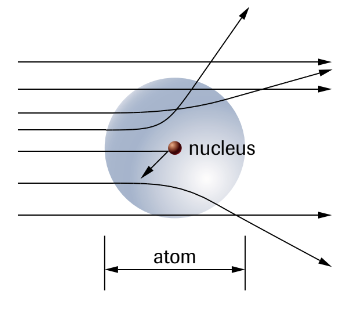
\includegraphics[width=0.4 \textwidth]{../figures/rutherford-experiment.png}
    \label{fig:rutherford-experiment}
\end{figure}

\newpage

\begin{figure}[ht!]
    \centering
    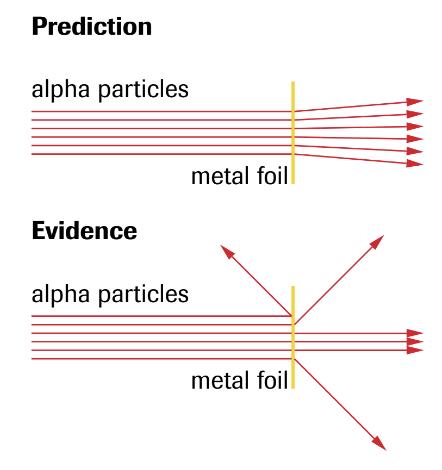
\includegraphics[width=0.4 \textwidth]{../figures/gold-foil-experiment.png}
    \caption{Prediction vs. Evidence: the particles were deflected at large angles instead of
    small angles}
    \label{fig:gold-foil-experiment}
\end{figure}

\begin{tabularx-custom}{|X X|}{Creating the Rutherford Atomic Theory (1911)}
    Key experimental work & Theoretical experiment \\ \hline
    Rutherford: a few positive particles are deflected at large angles when fired at a gold foil
                          & The positive charge in the atom must be very concentrated at a small
                          volume \\ \hline
    Most materials are very stable and do not fly apart (break down) & A very strong nuclear
    force holds the positive charges with the nucleus \\ \hline
    Rutherford: most alpha particles pass straight through the gold foil & Most of the atom is
    empty space \\ \hline
\end{tabularx-custom}

\subsection{Protons, Isotopes, and Neutrons}
Definitions:
\begin{bulleted-list}
    \item \textbf{Proton:} a positively charged subatomic particle found in the nucleus of atoms
    \item \textbf{Isotope:} a variety of atoms of an element; atoms of this variety have the
        same number of protons as all of the elements, but a different number of neutrons
    \item \textbf{Neutron:} a neutral/uncharged subatomic particle present in the nucleus of atoms
\end{bulleted-list}

\begin{bulleted-list}
    \item Previous studies by scientists found that the smallest positive charge possible was
        from ionized gas (leaving just the proton). This in turn became the \textbf{proton}
    \item By bending the hydrogen-gas positive rays in a magnetic field, they were able to 
        determine the charge and mass of the hypothetical proton
    \item The proton was shown to have a charge equal to but opposite to that of the electron
        and a mass 1836 times that of an electron
    \item Evidence from radioactivity and mass spectrometer falsified Dalton's theory that all
        atoms of a particular element were identical. There were actually \textbf{isotopes}
    \item James Chadwick used alpha particle bombardment to propose the existence of the
        \textbf{neutron}
\end{bulleted-list}

\begin{tabularx-custom}{|X X|}{Creating the concepts of protons, isotopes, and neutrons}
    Key experimental work & Theoretical explanation \\ \hline
    Rutherford (1914): the lowest charge on an ionized gas particle is from the hydrogen ion
    (the proton) & The smallest particle of positive charge is the proton \\ \hline
    Soddy (1913): radioactive decay suggest different atoms of the same element & Isotopes of
    an element have a fixed number of protons but varying stability and mass \\ \hline
    Aston (1919): mass spectrometer work indicates different masses for some atoms of the same
    element. See Figure \ref{fig:mass-spectrometer}.

    Chadwick: (1932): Radiation is produced by bombarding elements with alpha particles
                    & The nucleus contains neutral particles called neutrons \\ \hline
\end{tabularx-custom}

\begin{figure}[ht!]
    \centering
    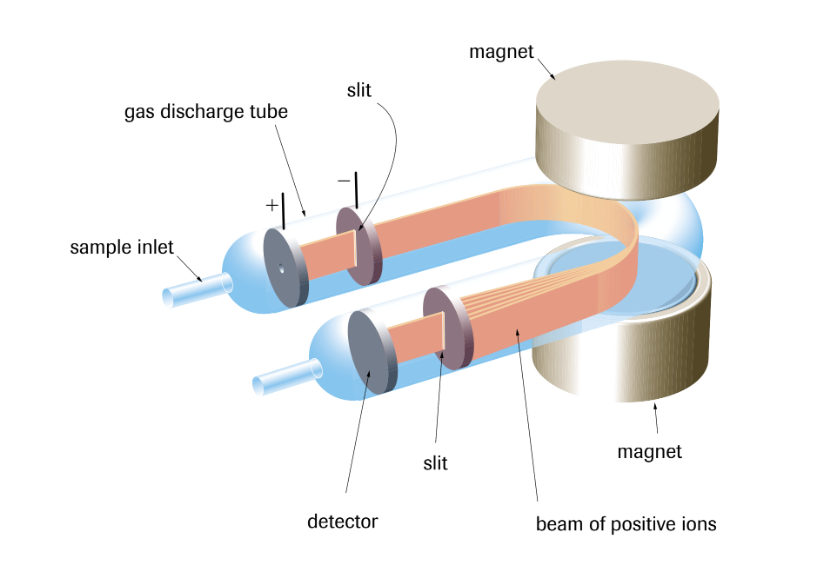
\includegraphics[width=0.7 \textwidth]{../figures/mass-spectrometer.png}
    \caption{A mass spectrometer is used to determine the masses of ionized particles by measuring
        the deflection of these particles as they pass through a strong magnet}
    \label{fig:mass-spectrometer}
\end{figure}

\begin{problems}
    \item Present the experimental evidence that led to the Rutherfor model
    \item How did Rutherford infer that the nucleus was
        \begin{enum-alph}
            \item very small (compared to the size of the atom)?
            \item positively charged?
        \end{enum-alph}
    \item
        \begin{enum-alph}
            \item State the experimental evidence that was used in the discovery of the proton
            \item Write a description of a proton
        \end{enum-alph}
    \item 
        \begin{enum-alph}
            \item State the experimental evidence that was used in the discovery of the neutron
            \item Describe the nature of the neutron
        \end{enum-alph}
    \item 
        \begin{enum-alph}
            \item State the experimental evidence that was used in the discovery of the neutron
            \item Describe the nature of the neutron
        \end{enum-alph}
    \item What is meant by a ``black box'' andw why is this an appopriate analogy for the study
        of atomic structure?
    \item Theories are often created by scientists to explain scientific laws and experimental
        results. To some people it seems strange to say that theories come after laws. Compare
        the scientific and common uses of the term ``theory''
\end{problems}

\begin{solutions}
    \item The gold foil experiment. As predicted, most of the $\alpha$-particles passed right through.
        However, some were deflected backwards, meaning that there was a densely positive center,
        called the nucleus
    \item 
        \begin{enum-alph}
            \item According to Dalton, some particles should be deflected at rather small angles.
                However, the particles were actually deflected at much larger angles than
                predicted. This means that the nucleus was very dense and small in volume
            \item The particles didn't pass through and were deflected
        \end{enum-alph}
    \item 
        \begin{enum-alph}
            \item In Figure \ref{fig:gold-foil-experiment}, you can see the prediction vs. evidence.
                The evidence was that some particles were deflected at large angles, and some
                even backwards
            \item The proton is a subatomic particle with a charge equal to but opposite to
                that of an electron and a mass of 1836 times greater
        \end{enum-alph}
    \item
        \begin{enum-alph}
            \item Chadwick used alpha particle bombardment to prove the existence of the neutron
            \item The proton is a neutral/uncharged subatomic particle present in the nucleus
                of atoms
        \end{enum-alph}
    \item The term ``black box'' refers to a system or object that can be understood and analyzed
        based on its inputs and outputs, regardless of its internal workings or structure.
        In the study of atomic structure, scientists could not directly observe the internal
        workings of an atom, but could analyze the results they presented. For instance, in
        Rutherford's gold foil experiment, they didn't know the internal workings of an atom,
        yet still proved the existence of a nucleus. Another example is Bohr's model; the model
        was based on the observed spectral lines of hydrogen--he could predict the behaviour of
        electrons in an atom without directly observing them
    \item Theories are scientific assumptions made based solely on previously proven knowledge,
        namely laws. Thus, it would be contradictory to assume that laws come after theories
        because there would be no laws to prove the pre-existing theories in the first place
\end{solutions}

\subsection{Case Study: A Canadian Nuclear Scientist}
An exceptional female student, who was Rutherford's first graduate student at McGill University,
is Canadian \textbf{Harriet Brooks}. Before the gold foil experiment, Rutherford was researching
radioactivity and invited Brooks. Brooks studied the reactivity of radium and found an ``emanation'',
which is radon from the radioactive decay of radium
\[
    \ch{^{226}_{86}Ra}\to \ch{^{222}_{86}Rn}+\ch{^{4}_{2}\alpha}
\]
\begin{bulleted-list}
    \item At the time, everyone believed that an element remained the same when it emitted radiation. Brookes
        disagreed and gathered evidence to falsify that claim
    \item Brooks used diffusion of the emanated gas to determine the molar mass of what we now
        know as radon
    \item In the process, she gathered evidence that led to Rutherford's theoretical interpretation
        that radiation resulted in the recoil (action-rejection) of the radiating nucleus. Often
        the recoiling nucleus was ejected from the radioactive sample
    \item Brook's third significant contribution was important evidence that Rutherford interpreted
        as a series of radioactive transformations. For example:
        \[
            \ch{^{226}_{86}Ra}\to \ch{^{222}_{86}Rn}\to \ch{^{218}_{84}Po}\to \ch{^{214}_{82}Pb}
        \]
        (emitting an alpha particle in each step)
\end{bulleted-list}

\begin{figure}[ht!]
    \centering
    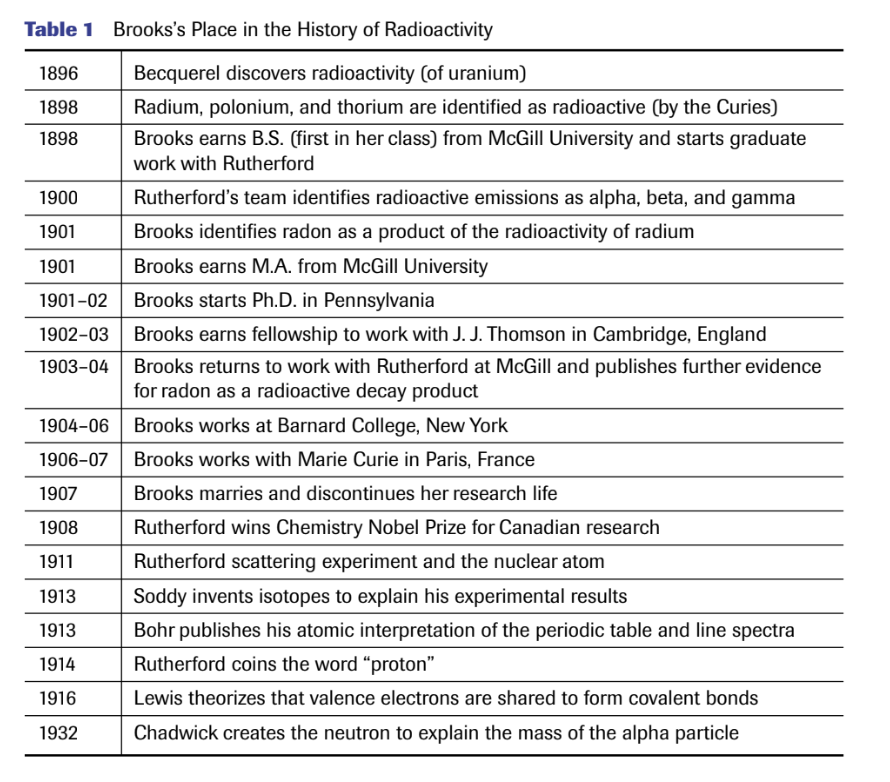
\includegraphics[width=0.9\textwidth]{../figures/history-of-radioactivity.png}
\end{figure}
